\documentclass[11pt, spanish]{article}
\usepackage[utf8]{inputenc}
\usepackage{listings} 
\usepackage{graphicx}
\usepackage{amsfonts}
\usepackage[dvipsnames]{xcolor}
\usepackage[T1]{fontenc}
\usepackage{bigfoot}
\usepackage{amsmath}
\usepackage[numbered,framed]{matlab-prettifier}
\usepackage{caption}
\usepackage[figurename=Figura, tablename=Tabla, font={small,tt}]{caption}
\usepackage{blkarray}
\usepackage{xcolor}
\usepackage{multicol}
\usepackage[]{algorithm2e}

\makeatletter
    \setlength\@fptop{0\p@}
\makeatother

\date{}

\usepackage{geometry}
 \geometry{
 a4paper,
 left=30mm,
 right=30mm,
 top=30mm,
 }

\lstset{
	style              = Matlab-editor,
  	basicstyle         = \mlttfamily,
  	escapechar         = ",
  	mlshowsectionrules = true,
	framesep=4.5mm,
	framexleftmargin=2.5mm,
	fillcolor=\color{White},
	rulecolor=\color{Black},
	numberstyle=\normalfont\tiny\color{Black}
}

\captionsetup[lstlisting]{font={small,tt}}
\renewcommand{\lstlistingname}{Script}
\newcommand\RED{\color{red}}
\newcommand\BLUE{\color{blue}}
\newcommand{\BigO}[1]{\ensuremath{\operatorname{O}\bigl(#1\bigr)}}
\newcommand{\norm}[1]{\left\lVert#1\right\rVert}

\begin{document}

\renewcommand\lstlistlistingname{Lista de Scripts}

\author{Sebastián Valencia Calderón \\ 201111578}
\title{Laboratorio 3: Algoritmos de Eliminación de Gauss con Pivoteo Parcial y Sustitución Regresiva}
\maketitle

%====================================================================
\section{Introducción}

Los sistemas de ecuaciones lineales, aparecen en una gran variedad de aplicaciones en ciencia e ingeniería. Su naturaleza algorítmica, da lugar al diseño de herramientas computacionales para hallar la solución de estos sistemas. Existen dos categorías de los métodos que solucionan estos sistemas de manera secuencial. Los métodos iterativos y los métodos directos. Métodos como el de Jacobi, o Gauss-Seidel, pertenecen a la primera categoría, mientras a la última, pertenecen métodos más naturales, como la eliminación Gaussiana. De los diferentes métodos, interesan la eficiencia, es decir, la velocidad de convergencia y la exactitud de la aproximación de esta respuesta.\\

Un sistema lineal, se puede describir a muy alto nivel como un conjunto de ecuaciones lineales en varias variables. Para estructurar mejor estos sistemas, se puede utilizar una matriz de valores $ A \in \mathbb{C}^{n \times m}$, un vector de incógnitas $\hat{x} \in \mathbb{C}^{m}$, y un vector de valores $\hat{b} \in \mathbb{C}^{n}$. De esta manera, se dispone la teoría de los espacios vectoriales y el calculo matricial para la solución de estos sistemas. A continuación, se incluye la forma en la cual resulta conveniente tratar estos sistemas. \\

$$
\begin{bmatrix} 
	a_{11} & a_{12} & \dots & a_{1n} \\ 
	a_{21} & a_{22} & \dots & a_{2n} \\
	\vdots & & & \vdots \\
	a_{m1} & a_{m2} & \dots & a_{mn}
\end{bmatrix} 
\times 
\left[ 
	\begin{array}{c} 
	x1 \\ 
	x2 \\
	\vdots \\
	xm 
	\end{array} 
\right] = 
\left[ 
	\begin{array}{c} 
	b1 \\ 
	b2 \\
	\vdots \\
	bn 
	\end{array} 
\right]
$$\\


La implementación de algoritmos, en una máquina digital, permite capacidades mayores en cuanto a la rapidez y recursos computacionales. Sin embargo, supone una severa restricción que proviene en la representación o aritmética de punto flotante. Es de crucial importancia plantear una metodología para medir el error en las respuestas de estas implementaciones. Asimismo, conviene comparar los diferentes métodos. En este caso en particular, se pretende estudiar a fondo la eliminación de Gauss con pivoteo parcial y sustitución hacia atrás, el estudio, se presenta usando \textsc{MATLAB} como herramienta y una metodología para medir los errores es presentada más adelante. Con el desarrollo de estos ejercicios, se pretende cumplir con los siguientes objetivos:

\begin{enumerate}
\item Reconocer algunos algoritmos de cómputo de soluciones de sistemas lineales.
\item Identificar casos de cómputo de matrices que requieren consideraciones respecto a la unidad de punto flotante de la máquina.
\item Reconocer casos de aplicación y los diversos métodos que ofrece \textsc{MATLAB} para solución de sistemas lineales.
\end{enumerate}

%==================================================================
\section{Procedimiento}

Para cumplir los objetivos enumerados anteriormente, se desarrollan algoritmos para resolver de manera directa sistemas de ecuaciones lineales, de manera específica, se desarrolla una función que implementa la eliminación de Gauss, creando los pivotes de la matriz $A$, además, se desarrolla un algoritmo para hallar la solución del sistema después de la eliminación de Gauss. Una vez los algoritmos están desarrollados y comprendidos, se procede a probarlos haciendo uso de un sistema lineal cuya solución analítica y algebraica es bien conocida, de tal manera que se puede comparar el resultado numérico obtenido a través de los algoritmos, y el valor conocido para distintos tamaños de la matriz. La comparación, se hace bajo un marco de referencia que permite medir la distancia de la solución obtenida con la real, métrica llamada error. Con base en la anterior descripción, se cuenta con una matriz $A$, y un vector $\hat{b}$, para los cuales existe un vector $\hat{x}$, cuya estructura y valor se conoce. Además se presentan, un algoritmo para reducir el sistema a un estado donde resulta trivial su solución, un algoritmo que aprovecha esta trivialidad y resuelve el sistema, y una metodología para medir el error de la solución. A lo largo de este proceso, se estudian detalladamente la matriz y los algoritmos. \\

Una vez se tenga comprensión de estos conceptos y de la geometría de las soluciones propuestas, se aplican los algoritmos para resolver sistemas de ecuaciones lineales que surgen en la vida real, de manera más específica, en la solución de circuitos lineales de naturaleza resistivos, donde se sabe que se trabaja con sistemas de ecuaciones lineales de a veces muchas variables. Este resultado, y aplicación, resulta útil para la simulación de circuitos, técnica ampliamente usada en la industria.


%==================================================================
\section{Resultados}

A continuación, se exponen los resultados, las metodologías propuestas para los análisis y las herramientas de ejecución para cada uno de los problemas propuestos.\\

\begin{enumerate}
\item Se implementan en \textsc{MATLAB} algoritmos, uno para la eliminación de Gauss con pivoteo parcial y otro para la sustitución hacia atrás. Para garantizar un entendimiento completo y detallado, se incluye a continuación,  la deducción de los algoritmos. 

\begin{itemize}
\item \textbf{Sustitución hacia atrás.} Ocasionalmente, la estructura de una matriz, permite facilidades para computar el vector respuesta de un sistema de ecuaciones lineales dispuesto en forma matricial. Una instancia estructural de una matriz de interés en el caso presente, es el de las matrices con estructura superior triangular, es decir, matrices cuadradas para las cuales las entradas inferiores a la diagonal, son necesariamente cero, es decir, una matriz es superior triangular sí y sólo si, se tiene:


\begin{multicols}{2}
  $$
  A_{ij} =
  \begin{cases}
    a_{ij} & \text{si } i \leq j \\
    0 & \text{de lo contrario}
  \end{cases} 
$$\break
  $$A = 
\begin{blockarray}{ccccc}
\begin{block}{[ccccc]}
 a_{11} & \BLUE a_{12} & \BLUE a_{13} & \BLUE ... & \BLUE a_{1n} \\
 \RED 0 & a_{22} & \BLUE a_{23} & \BLUE ... &  \BLUE a_{2n} \\
 \RED 0 & \RED 0 & a_{33} &  \BLUE... & \BLUE a_{3n} \\
 \RED \vdots & \RED \vdots &\RED \vdots & \vdots & \BLUE \vdots\\
 \RED 0 & \RED 0 & \RED 0 & \RED ... & a_{nn} \\
\end{block}
\end{blockarray}$$
\end{multicols}

En este caso, cada ecuación, depende del valor próximo, es decir, para obtener el valor $x_k$, es necesario saber los valores $\{x_{k+1},\ x_{k + 2},\ \dots,\ x_{n} \}$, por lo que resulta necesarios, comenzar por $x_{n}$, cuyo alor, se obtiene de forma directa, pues $x_n = \frac{b_n}{a_{nn}}$, ahora, una vez se conoce el valor de $x_n$, es posible conocer el valor de $x_{n-1}$, y así sucesivamente, de manera general, se tiene la siguiente igualdad:

$$x_{k} = \frac{b_{k} - \sum_{j = k + 1}^{n}\left[ a_{kj} \times x_j\right]}{a_{kk}}\ k \in \{ 1,\ 2,\ \dots,\ n \}$$

Esto da lugar, a plantear el siguiente algoritmo:\\

\begin{algorithm}[H]
 \KwData{$A \in \mathbb{R}^{n \times n}$, tal que $A$ es triangular superior.\\ $a_{ii} \neq 0\ \forall i \in \{ 1,\ \dots ,\ n \}$}
 \KwData{Un vector $b \in \mathbb{R}^n$}
 \KwResult{Un vector $x$ tal que $A \times x = b$}\
 
 \For{$k \in [n,\ n - 1,\ \dots,\ 1]$}{
 $x_{k} = \frac{b_{k} - \sum_{j = k + 1}^{n}\left[ a_{kj} \times x_j\right]}{a_{kk}}$
 }\
 \caption{Sustitución hacia atrás para sistemas lineales.}
\end{algorithm}\

Una formulación más natural, que brinda claridad para analizar el algoritmo, es la siguiente:\\

\begin{algorithm}[H]
 \KwData{$A \in \mathbb{R}^{n \times n}$, tal que $A$ es triangular superior.\\ $a_{ii} \neq 0\ \forall i \in \{ 1,\ \dots ,\ n \}$}
 \KwData{Un vector $b \in \mathbb{R}^n$}
 \KwResult{Un vector $x$ tal que $A \times x = b$}\
 
 \For{$k \in [n,\ n - 1,\ \dots,\ 1]$}{
 	$x_{k} \gets b_k$\\
 	 \For{$j \in [k+1,\ \dots,\ n]$}{
 	 	$x_k = x_k - a_{kj} \times x_j$
	 }
	 $x_k = x_k / a_{kk}$
 }\
 \caption{Sustitución hacia atrás para sistemas lineales.}
\end{algorithm}

\newpage

El costo computacional de este algoritmo, es:

$$C = \sum_{k = 1}^{n} \left[ 1 + \left[\sum_{j = k +1}^{n} \BigO{1} \right] + 1\right] = 
\sum_{k = 1}^{n} \left[ 1 + \left[n + \BigO{1} - (k + 1) \right] + 1\right]$$
$$\sim \sum_{k = 1}^{n} \left[ 1 + n - k + 1\right] \sim \sum_{k = 1}^{n} \left[n - k + \BigO{1} \right] \sim \sum_{k = 1}^{n}  n  + \sum_{k = 1}^{n} 1 - \sum_{k = 1}^{n} k\sim \BigO{n^2}$$\\

El script \ref{lst:back_substitution}, posee la implementación de la sustitución hacia atrás, haciendo uso del primer algoritmo (es necesario resaltar que $\sum_{j = k + 1}^{n}\left[ a_{kj} \times x_j\right]$, puede ser visto como un producto punto, resultado que se usa en la implementación en \textsc{MATLAB}). Una aproximación más práctica a este algoritmos y la deducción, se encuentra en la referencia \cite{ascher2011numerical}. La implementación en \textsc{MATLAB}, se encuentra en la referencia \cite{mathews1999matlab}. \\

\item \textbf{Eliminación de Gauss con pivoteo parcial.} La estructura de una matriz, no siempre se presta para ser aprovechada en la solución de un sistema de ecuaciones lineales. La eliminación de Gauss, sirve para llevar un sistema de ecuaciones lineales, a una forma donde $A$ sea una matriz triangular superior y $b$, refleje las transformaciones del sistema, esto siempre y cuando $A$ sea una matriz no singular. La deducción de este algoritmo, no es tan intuitiva. Por lo tanto, no se incluye la deducción del algoritmo. Sin embargo, la técnica consiste en aplicar de manera sucesiva hasta lograr la forma deseada las siguientes transformaciones en el orden mas conveniente:

\begin{itemize}
\item Cualquier par de filas, pueden ser intercambiadas. $R_i \longleftrightarrow R_j$, significa que las filas $i$ y $j$ son intercambiadas de posición.
\item Cualquier fila, puede ser escalada por un escalar cualquiera. En este caso, lo llamaremos $\alpha$. $R_i \longleftarrow \alpha \times R_i$, significa que la fila $i$, se convierte en la fila por $\alpha$.
\item Cualquier múltiplo de una fila, puede ser sumado a otra fila. $R_i \longleftarrow R_i + \alpha \times R_j$, significa que $\alpha$ veces el vector file $R_j$, es sumado al vector fila $R_i$, y este último es reemplazo por este valor.
\end{itemize}

Haciendo uso de estas transformaciones, se obtiene la idea tras la eliminación de Gauss con pivoteo parcial: intercambiar filas en cada paso dela eliminación de Gauss, poniendo el mayor elemento de cada columna en la diagonal de la matriz aumentada de la forma $[A\ |\ b]$. Los intercambios pertinentes, se llevan a cabo haciendo uso de intercambios de matrices $R_i \longleftrightarrow R_k$, donde $a_{ki}$, es el elemento de mayor valor bajo o sobre la diagonal de la $i$-ésima columna, es decir, $|a_{ki}| = \max{|a_{ji}|}\ j \in \{i \dots n\}$. El proceso computacional, haciendo uso de transformaciones auxiliares provistas a partir de operaciones auxiliares, se explica claramente en las referencias: \cite{datta1995numerical}, y \cite{golub2012matrixcomputations}. La última referencia, propone el siguiente algoritmo para la eliminación de Gauss con pivoteo parcial de una matriz A:

\begin{algorithm}[H]
 \KwData{$A \in \mathbb{R}^{n \times n}$, tal que $A$ es invertible.}
 \KwResult{$A \in \mathbb{R}^{n \times n}$, tal que $A$ es triangular superior.\\ $a_{ii} \neq 0\ \forall i \in \{ 1,\ \dots ,\ n \}$}\
 
 \For{$k \in [1,\ 2,\ \dots,\ n]$}{
 Encontrar una matriz e permutación $\Pi_k \in \mathbb{R}^{n \times n}$\\
 que intercambie $a_{kk}$ con el mayor elemento de la\\ $k$-ésima columna de $A$\\
 	$A \gets \Pi_{k} \times A$\\
 	Determinar la trasformación de Gauss $M_k = I_n - \tau^{(k)} \times e_{k}^T$\\
 	de manera que se deje la $k$-ésima columna de $A$, desde la\\ posición $k+1$ en adelante
 	en cero.\\
	$A \gets M_{k} \times A$\\
 }\
 \caption{Pivoteo parcial haciendo uso de matrices $\Pi_k$ y $M_k$}
\end{algorithm}\


El algoritmo anterior, se implementa y documenta en el script \ref{lst:gaussian_elimination}.

\end{itemize}

\item Para validar los algoritmos implementados, se propone el uso de la matriz de Hilbert de orden $n$, para resolver el sistema $A \times x = b$. $A$ es unamatriz de Hilbert y $b$, es un vector definido de tal manera que $x$, es el vector que satisface $x_i = i;\ \forall\ i \in \{1 \dots n\}$. Las definiciones de la matriz y el vector, se anotan a continuación (en el contexto de las siguientes ecuaciones, $i,\ j = 1\ \dots\ n$):

\begin{multicols}{2}
  $$
  b_{i} = \sum_{k = 1}^{n} \frac{k}{i + k - 1}
$$\break
$$  
  A_{ij} = \frac{1}{j + i - 1}
$$   
\end{multicols}

$$A_n = H_n = \begin{bmatrix}
    1 & \frac{1}{2} & \frac{1}{3} & \dots  & \frac{1}{n} \\
    \frac{1}{2} & \frac{1}{3} & \frac{1}{4} & \dots  & \frac{1}{n + 1} \\
    \vdots & \vdots & \vdots & \ddots & \vdots \\
    \frac{1}{n} & \frac{1}{n+1} & \frac{1}{n+2} & \dots  & \frac{1}{2n - 1}
\end{bmatrix}$$\

La generación de estas matrices, se implementa  en el script \ref{lst:generate_system}. Ahora, se cuenta con una matriz $A$ y un vector $b$, para los cuales se conoce que la respuesta analítica o algebraica del sistema de ecuaciones lineales $Ax = b$, es un vector $x \in \mathbb{R}^n$ tal que $x_i = i$, y además, con un algoritmo para convertir un sistema en uno con matriz $A$ triangular superior, y un algoritmo que resuelve el sistema explotando la estructura de las matrices de este tipo. Ahora, se estudia el error o la perturbación de estas matrices con respecto a las soluciones de los sistemas, es decir, el error y el residuo de las soluciones. Para medir la distancia entre dos vectores, se hace uso de la norma en $\mathbb{R}^n$. Las propiedades y deducciones importantes, han sido estudiadas de \cite{bradie2006friendly}. 

$$\norm{.}\ : \mathbb{R}^n \longrightarrow \mathbb{R}\ |\ \norm{x} = \sqrt{x^Tx} = \sqrt{\sum_{i = 1}^{n}x_i^2}$$

Entonces, medir el error, se usa $e = \norm{\hat{x} - x}$. El residuo es $\norm{A\hat{x} - b}$. Una forma sugerida para medir el error en el caso presente, es $\norm{A\hat{x} - b} / \norm{x}$.\\

El script \ref{lst:validate}, calcula las matrices $A$ y $b$ (haciendo uso del script \ref{lst:generate_system}), ejecuta eliminación Gaussiana sobre el sistema aumentado $[\ A\ |\ b\ ]$ (haciendo uso del script \ref{lst:gaussian_elimination}), y calcula la solución numérica al sistema (haciendo uso del script \ref{lst:back_substitution}). A continuación, se muestran algunas matrices de Hilbert, los vectores asociados y la solución usando las funciones \texttt{gaussianelimination()} y \texttt{backsubstitution()}.  La ejecución de \texttt{validate(3)}, arroja los siguientes resultados:

$$A = \left(\begin{array}{ccc} 1 & \frac{1}{2} & \frac{11184811}{33554432}\\ \frac{1}{2} & \frac{11184811}{33554432} & \frac{1}{4}\\ \frac{11184811}{33554432} & \frac{1}{4} & \frac{13421773}{67108864} \end{array}\right)
 b = \left(\begin{array}{c} 3\\ \frac{16078165}{8388608}\\ \frac{12023671}{8388608} \end{array}\right) x = \left(\begin{array}{c} 1\\ 2\\ 3 \end{array}\right)$$


Posteriormente, se procede a medir el error para varios valores de $n$. Ya que se incluyó el error en el script \ref{lst:gaussian_elimination}, la función del script \ref{lst:validate}, no se ejecutará si la matriz es singular. Para medir el error en función de $n$, se calcula el valor $\hat{n}$, para el cual la matriz de Hilbert posee problemas para la solución del sistema, esto por errores de redondéo y representación interna en el computador. Luego, se ejecuta \texttt{validate()}, y se compara el $x$ arrojada por esta, con el valor de la solución analítica del sistema ($x_i = i$). Todo este proceso, es ejecutado en el script \ref{lst:simulation}. A continuación, se muestra el resultado obtenido.

\begin{figure}[htbp]
\centering
	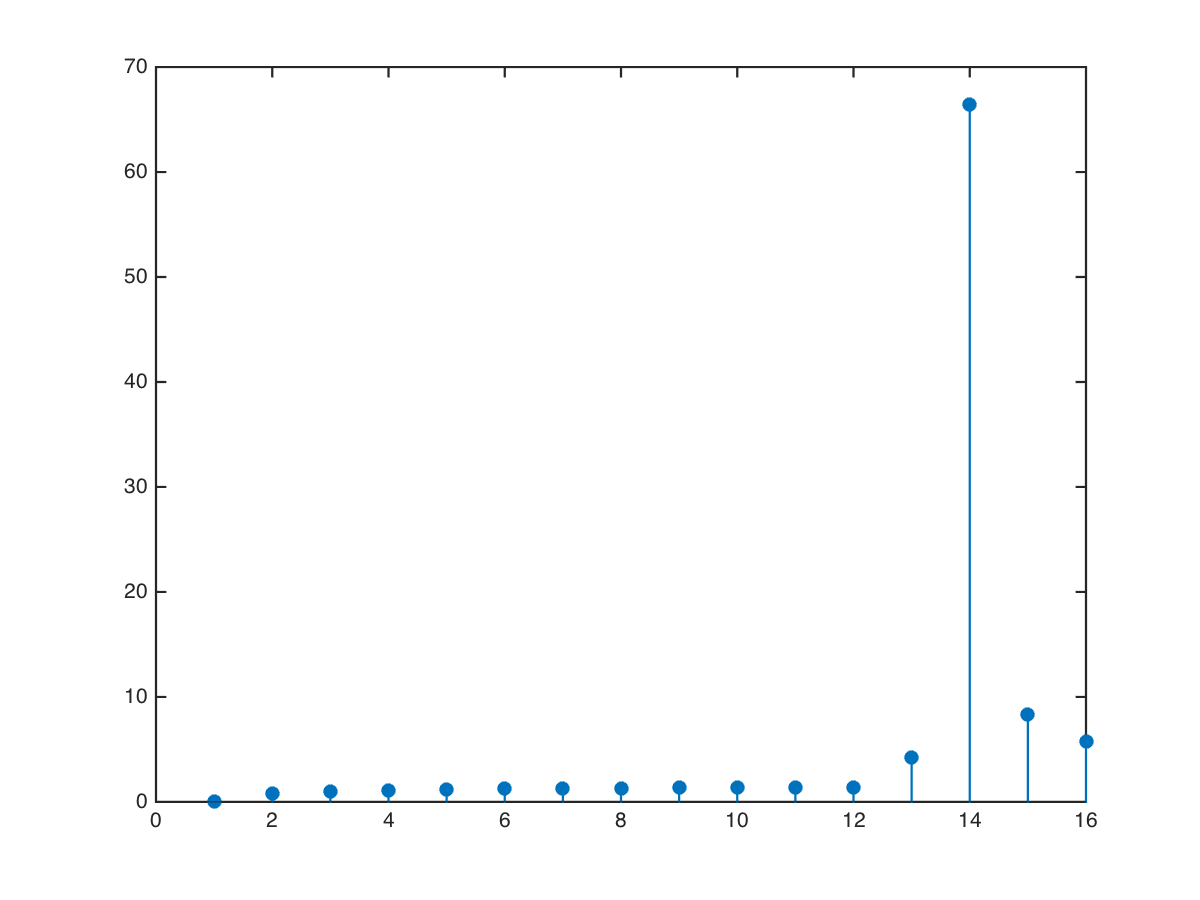
\includegraphics[scale=0.55]{data/img/error}
	\caption{Errores obtenidos con la solución numérica y la algebraica de cada sistema para un orden o tamaño variante. El eje x es el tamaño del problema, y el y el error absoluto medido.}
\end{figure}

El vector de errores asociados al calculo documentado anteriormente es:
\begin{align*}
[0,\ 0.75899,\ 0.98478,\ 1.10780,\ 1.18572,\ 1.23971,\ 1.27945,\ 1.31001,\\ 1.33430,\ 1.35410,\ 1.37060,\ 1.38667,\ 4.21665,\ 66.47713,\ 8.28886,\ 5.75513]
\end{align*}

Dado que la matriz de Hilbert, posee elementos en la diagonal cada vez más cercanos a cero, el pivote, por el cual se divide en la eliminación Gaussiana, causa una perturbación que se desplaza hasta afectar la solución del sistema, esto se evidencia por el hecho, de que la matriz se vuelve numéricamente singular cuando n tiende a un tamaño grande, y por que en los valores menores a $\hat{n}$, entre mayor sea el número, mayor es el error.

\item Para aplicar la teoría en un caso real, se tiene un circuito, para el cual es necesario hallar las corrientes y voltajes para cada uno de los elementos pasivos. Se sabe que la solución de las corrientes o voltajes de muchos de estos circuitos lineales resistivos, se obtiene a partir de la solución de un sistema de ecuaciones lineales.

\begin{figure}[htbp]
\centering
	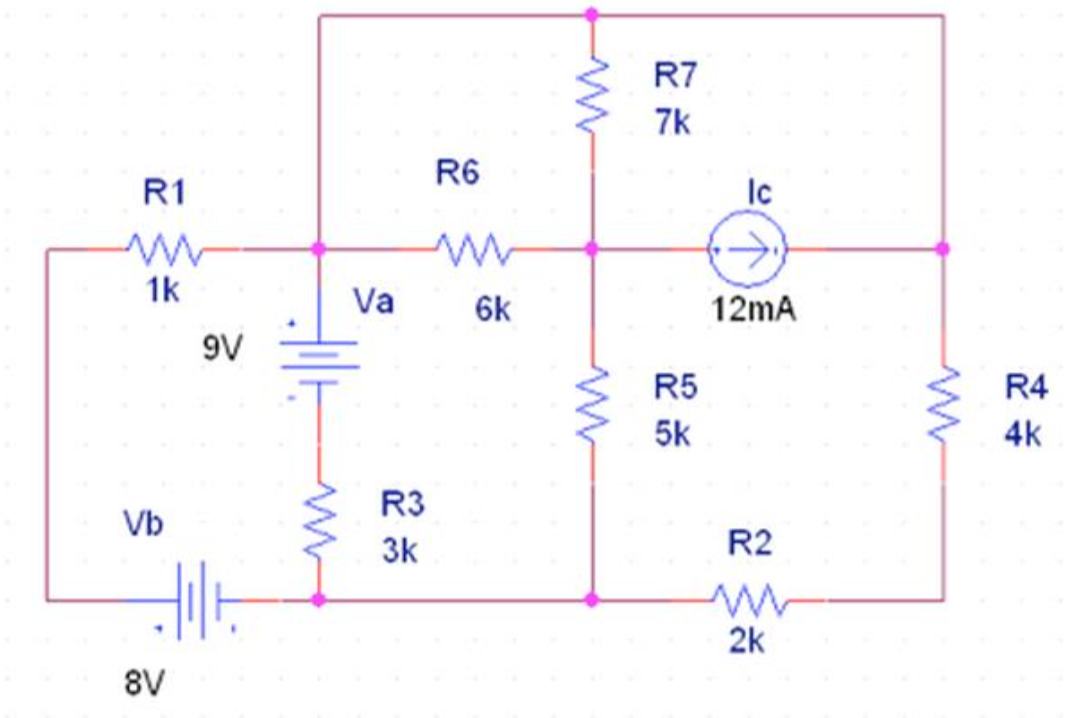
\includegraphics[scale=0.55]{data/img/circuit}
	\caption{Circuito a resolver.}
\end{figure}

Para resolver este circuito, se emplea la técnica de análisis de lazo y superlazo. Esta técnica, se encuentra debida y sucintamente documentada en la referencia \cite{valkenburg1999circuits}.\\

\begin{tabular}{ |l|l| }
  \hline
  \multicolumn{2}{|c|}{Corrientes por lazo propuestas para resolver el circuito de la figura.} \\
  \hline
  $I_1$ & Corriente en el lazo que contiene la fuente de voltaje $V_b$, $R_1$, $V_a$, y $R_3$ \\
  $I_2$ & Corriente en el lazo que contiene la fuente de voltaje $V_a$, $R_6$, $R_5$, y $R_3$ \\
  $I_3$ & Corriente en el lazo que contiene la fuente de corriente $I_c$, $R_4$, $R_2$, y $R_5$ \\
  $I_4$ & Corriente en el lazo que contiene $R_6$,  y $R_37$ \\
  $I_5$ & Corriente en el lazo que contiene la fuente de corriente $I_c$,  y $R_7$ \\
  \hline
\end{tabular}\\

La corriente del super lazo, recorre los elementos $R_2$, $R_5$, $R_7$, y $R_4$, de tal manera, se tiene la siguiente igualdad por leyes de Kirchoff, $I_3 = I_c + I_5$. Las otrás ecuaciones, se obtienen por el análisis aplicado sin mayor sofisticación.

\begin{align*}
V_b = I_1 R_1 + V_a + R_3(I_1 - I_2)\\
V_a = R_6(I_2 - I_4) + R_5(I_2 - I_3) + R_3(I_2 - I_1)\\
I_3 = I_c + I_5\\
0 = I_3R_2 + R_5(I_3 - I_2) + R_7(I_5 - I_4) + R_4 I_3\\
0 = R_6(I_4 - I_2) + R_7(I_4 - I_5)
\end{align*}\

Las ecuaciones se agrupan, y se obtiene el siguiente sistema de ecuaciones lineales:

\[
\begin{bmatrix}
    R_1 + R_3 & -R_3 & 0 & 0  & 0 \\
    -R_3 & R_6 + R_5 + R_3 & -R_5 & -R_6  & 0 \\
    0 & 0 & 1 & 0  & -1 \\
    0 & -R_5 & R_2 + R_5 + R_4 & -R_7  & R_7 \\
    0 & -R_6 & 0 & R_6 + R_7  & -R_7
\end{bmatrix} \times \begin{bmatrix}
    I_1 \\
    I_2 \\
    I_3 \\
    I_4 \\
    I_5
\end{bmatrix} = \begin{bmatrix}
    V_b - V_a \\
    V_a \\
    I_c \\
    0 \\
    0
\end{bmatrix}
\]

La realización de este sistema para el caso que nos ocupa, es:

\[
\begin{bmatrix}
    4000 & -3000 & 0 & 0  & 0 \\
    -3000 & 14000 & -5000 & -6000  & 0 \\
    0 & 0 & 1 & 0  & -1 \\
    0 & -5000 & 11000 & -7000  & 7000 \\
    0 & -6000 & 0 & 13000  & -7000
\end{bmatrix} \times \begin{bmatrix}
    I_1 \\
    I_2 \\
    I_3 \\
    I_4 \\
    I_5
\end{bmatrix} = \begin{bmatrix}
    -1 \\
    9 \\
    0.012 \\
    0 \\
    0
\end{bmatrix}
\]

Para resolver el sistema, se hace uso de las funciones programadas en \textsc{MATLAB}, y las funciones programadas en el literal anterior. Las funciones a usar y su metodología es:\\

\begin{itemize}
\item Eliminación Gaussiana y sustitución regresiva (scripts \ref{lst:gaussian_elimination} y \ref{lst:back_substitution}). Usan la metodología expuesta anteriormente, la cual se dedujo y documentó en el literal uno de esta sección. 

\item \texttt{inv(A) * b'}, el objetivo de esta expresión, es hallar la inversa de una matriz $A$, y multiplicar $A^{-1}$ y el vector $b$, para obtener el valor del vector $x$. El único parámetro de \texttt{inv()}, es la matriz a invertir, este no se implementa, reduciendo el sistema aumentado $[\ A\ |\ b\ ]$, y aplicando eliminación de Gauss, pues \textsc{MATLAB}, documenta demoras en la aplicación de esta función para resolver un sistema, pues interviene ademas, la multiplicación de matrices (\BigO{n^3 }).

\item \texttt{linsolve()}, recibe como parámetros la matriz $A$, y el vector $b$. Su funcionamiento, fue explicado anteriormente.

\item \texttt{rref()}, recibe como parámetro el sistema aumentado $[\ A\ |\ b\ ]$, y aplicando eliminación de Gauss, determina la forma escalonada reducida para obtener las respuestas requeridas.

\item \texttt{mldivide()}, recibe como parámetro la matriz $A$, y el vector $b$. Aplicando optimización de mínimos cuadrados, este llega a la respuesta en el caso de que $A$ sea no singular.
\end{itemize}

El script \ref{lst:circuit}, muestra el procedimiento para obtener el vector de corrientes requerido. A continuación, se muestran los valores del vector de corrientes, usando cada uno de los métodos propuestos.

\begin{figure}[htbp]
\centering
	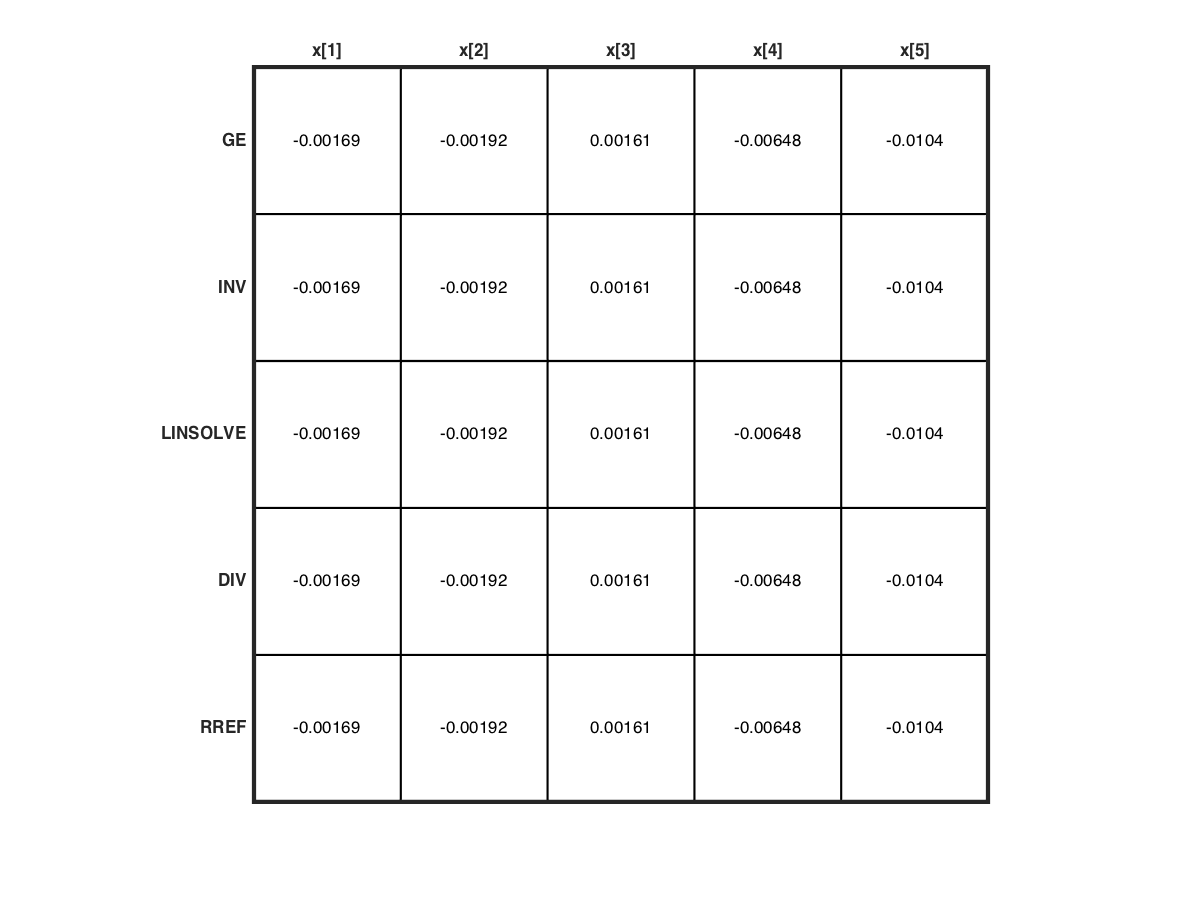
\includegraphics[scale=0.7]{data/img/plot_circuit_solution}
	\caption{Vector de corrientes haciendo uso de los métodos propuestos y documentados anteriormente}
\end{figure}

Como puede verse, todos los métodos, llegan a una solución, por el consenso evidenciado entre ellos, se puede ver que todos los métodos son útiles para hallar el resultado de un sistema de ecuaciones lineales. En un problema bien condicionado, se debe explorar la estructura de la matriz y elegir el método mas conveniente según la misma estructura, lo cual puede llevar a mejoras computacionales significativas.\\

Valores de las corrientes por cada lazo propuestas para resolver el circuito de la figura anteriormente:

\begin{center}
\begin{tabular}{ |l|l| }
  \hline
  $I_1$ & -1.69 mA \\
  $I_2$ & -1.92 mA \\
  $I_3$ & 1.61 mA\\
  $I_4$ & -6.48 mA \\
  $I_5$ &  -10.4 mA\\
  \hline
\end{tabular}
\end{center}

El voltaje de $R_1$, es $1000 \times I_1$. El voltaje de $R_2$, es $2000 \times I_3$, el voltaje de $R_3$, es $3000 \times (I_1 - I_2)$. El voltaje de $R_4$ es $4000 \times I_3$. El voltaje de $R_5$, es $5000 \times (I_2 - I_3)$. Los voltajes de $R_6$ y $R_7$, son respectivamente $6000 \times (I_4 - I_2)$ y $7000 \times (I_4 - I_5)$.




\end{enumerate}

%==================================================================
\section{Conclusiones}

Mediante el desarrollo del laboratorio propuesto, se pudo verificar la importancia del diseño y análisis de algoritmos, en el álgebra lineal numérica o cálculo o álgebra matricial. Conocer algoritmos para resolver sistemas de ecuaciones lineales, permite hacer uso de máquinas digitales para implementar, obtener y verificar la solución de sistemas de ecuaciones lineales. Además de ver esto, se estudió la gran variedad de algoritmos existentes para las soluciones de estos sistemas; se identificaron casos que requieren consideraciones más allá de meter los datos en un computador, y esperar que un algoritmo los resuelva, se observó la relación del error con el tamaño y condicionamiento de los problemas, las restricciones analíticas de los algoritmos, y la utilidad de lo implementado a casos específicos de ingeniería electrónica. De manera más específica, y en relación con los problemas tratados, se concluye lo siguiente

\begin{itemize}
  \item Es necesario contar con sólida bases para entender de manera intuitiva, el comportamiento de las matrices, su estructura y geometría, asi como entender de manera intuitiva, los algoritmos, lo que implica conocer su uso, su poder, su eficiencia y sus restricciones. El conocimiento de la representación de los números en una máquina, permite inferir el comportamiento de los algoritmos sobre problemas en específico.\\
  
  En el caso tratado en particular, se sabe que las matrices de Hilbert, están mal condicionadas con un $n$ grande (dependiendo de los recursos computacionales dispuestos para los cálculos), por lo cual, un algoritmo así sea verificado de manera formal y con las mejores bases teóricas, como la aplicación secuencial de la eliminación de Gauss y la sustitución regresiva, puedan presentar problemas para hallar una solución estable y precisa. Por lo tanto, conviene estudiar el condicionamiento de los problemas y de las matrices en ellos comprometidas para realizar cálculos numéricos mas preocupados o sofisticados. A parte de esto, conviene estudiar mas a fondo esta representación, y algunas estrategias para mitigar este tipo de errores, pues los errores imperceptibles, pueden tener fatales consecuencias en las aplicaciones de estos sistemas lineales en sistemas reales de alto impacto. Es necesario, comprometerse con otras estrategias como la representación a través de listas o evaluación perezosa de expresiones (aritmética de precision infinita en lenguajes puramente funcionales)
  
   \item La implementacion de algoritmos para la solución de sistemas lineales bien condicionados, resulta muy conveniente para la practica. Bien es sabido que los sistemas de ecuaciones lineales, aparecen en problemas de circuitos, de mecánica, de control, de procesamiento de señales, y son la base o la piedra angular de los métodos numéricos. Resulta muy practico y útil contar con herramientas de simulación para cada área en especifico,  un lenguaje para expresar las operaciones matriciales de manera conveniente, y una arquitectura de computador que permita la manipulación y operación efectiva de matrices.
   
   \item Las convenciones analíticas o algebraicas pero de todos modos teóricas de las matemáticas aplicadas, distan mucho de las usadas en la practica, donde es necesarios hacer uso de maquinas digitales que soporten el proceso de computo de los valores, lo que resulta en una restricción grande, pero que ha permitido avanzar la humanidad en varias áreas del conocimiento.
\end{itemize}


%==================================================================
\newpage
\section{Bibliografía}

\begingroup
\renewcommand{\section}[2]{}%
\begin{thebibliography}{}

  \bibitem{bradie2006friendly} Bradie, B. {\em A Friendly Introduction to Numerical Analysis.}  2006. Pearson Prentice Hall - Featured Titles for Numerical Analysis Series. Página 150 - 174.
  
  \bibitem{valkenburg1999circuits} Van Valkenburg, M. E. {\em Análisis de Redes.}  1999. Limusa. Página 86 - 92.
  
  \bibitem{ascher2011numerical} Ascher, U. M, Greif, C. {\em A First Course in Numerical Methods.}  2011. Society for Industrial \& Applied Mathematics - Computational Science and Engineering. Página 93- 108.
  
  \bibitem{golub2012matrixcomputations} Golub, G. H, Van Loan, C. F. {\em Matrix Computations.}  2012. Johns Hopkins University Press - Johns Hopkins Studies in the Mathematical Sciences.
  
   \bibitem{datta1995numerical} Datta, B. N. {\em Numerical Linear Algebra and Applications.}  1995. Brooks-Cole Pub Co.
   
   \bibitem{vanloan1996matlab} Van Loan, C. F. {\em Introduction to Scientific Computing: A Matrix-Vector Approach Using MATLAB.}  1996. Brooks-Cole Pub Co.
    
    \bibitem{mathews1999matlab} Mathews, J. H, Fink, K. K. {\em Numerical Methods Using Matlab}  1999. Prentice Hall.

\end{thebibliography}
\endgroup

%==================================================================
\newpage
\section{Scripts}

\lstinputlisting[caption = {Sustitución regresiva.}, label={lst:back_substitution}]{data/scripts/back_substitution.m}

\lstinputlisting[caption = {Eliminación Gaussiana.}, label={lst:gaussian_elimination}]{data/scripts/gaussian_elimination.m}

\lstinputlisting[caption = {Generación de la matriz de Hilbert de ordern n, y del vector acompañante.}, label={lst:generate_system}]{data/scripts/generate_system.m}

\newpage

\lstinputlisting[caption = {Calcula las matriz de Hilbert y el vector correspondiente de orden n (haciendo uso del script \ref{lst:generate_system}). Ejecuta eliminación Gaussiana sobre el sistema aumentado (haciendo uso del script \ref{lst:gaussian_elimination}), y calcula la solución numérica al sistema (haciendo uso del script \ref{lst:back_substitution}). Usa precisión simple a través de la función de MATLAB single().}, label={lst:validate}]{data/scripts/validate.m}

\lstinputlisting[caption = {Simulación de validate(), para varios valores de n. Obtención del error a partir del valor calculado por validate(), y la solución algebraica.}, label={lst:simulation}]{data/scripts/simulation.m}

\lstinputlisting[caption = {Solución del circuito, haciendo uso de varios métodos.}, label={lst:circuit}]{data/scripts/circuit.m}




\addcontentsline{toc}{chapter}{\lstlistlistingname}
\lstlistoflistings

\bibliography{sample}

\end{document}
